%% Journal of Theoretical Biology (Elsevier) -- preprint format.
%% Compile: pdflatex twice. Requires elsarticle.cls (texlive-publishers).
%% Elsevier accepts format-free initial submission; to fall back to a
%% standard class, replace the \documentclass line with
%%   \documentclass[11pt]{article}
%% and delete the \begin{frontmatter}...\end{frontmatter} block in favour
%% of \maketitle.

\documentclass[preprint,11pt]{elsarticle}

\usepackage[T1]{fontenc}
\usepackage{amsmath,amssymb,amsthm}
\usepackage{booktabs}
\usepackage{graphicx}
\usepackage[expansion=false]{microtype}
\usepackage{xcolor}
\usepackage[colorlinks=true,linkcolor=blue!55!black,citecolor=blue!55!black,
            urlcolor=blue!55!black]{hyperref}

\newtheorem{proposition}{Proposition}
\newtheorem{corollary}[proposition]{Corollary}
\theoremstyle{remark}
\newtheorem{remark}[proposition]{Remark}

\newcommand{\Rpos}{\mathbb{R}_{>0}}
\newcommand{\gateset}{\mathcal{G}}

\journal{Journal of Theoretical Biology}

\begin{document}

\begin{frontmatter}

\title{Symmetric rate perturbations of Hodgkin--Huxley gating are
observationally equivalent: an identifiability constraint on
mechanosensitivity experiments}

\author{Duston Moore}
\ead{dhwcmoore@gmail.com}
\address{Independent Researcher, Edmonton, Alberta, Canada}

\begin{abstract}
Mechanical modulation of voltage-gated channel kinetics is usually represented
in Hodgkin--Huxley models by multiplying the forward and reverse rates of a gate
by a common strain-dependent factor. We show that this representation carries
strictly less information than it appears to. For an arbitrary compartmental
Hodgkin--Huxley system, the solution operator depends on the perturbation
parameters only through the vector of rate multipliers, so every pair of
mechanistic stories that induces the same multipliers defines the identical
dynamical system, and hence the identical voltage trajectory, under every
stimulus and every initial condition. Three
consequences follow. First, the coupling coefficient and the imposed strain are
not separately identifiable from a single strain level; only their product is.
Second, a spatially and gate-uniform strain perturbation is indistinguishable
from the kinetic component of a temperature change: a reported 1.4-fold
acceleration is reproduced exactly by a rise of $3.06\,^{\circ}$C at
$Q_{10}=3$. Third, no measurement of the membrane-voltage trajectory, however
detailed, can separate them, so agreement between a strain-coupled model and a
recorded spike waveform is not evidence of mechanical coupling. We then identify
what does discriminate. The gate-selective component of the log-multiplier
vector is identifiable and is not produced by uniform thermal scaling; the
symmetric-scaling hypothesis predicts a voltage-independent log ratio of
relaxation times together with an unshifted steady-state activation curve,
which separates it from effective-voltage coupling; and areal strain and warming
act on channel surface density with opposite sign, predicting a divergence of
$8$ to $24\%$ in peak conductance at the reference perturbation whose sign does
not depend on the poorly constrained conductance $Q_{10}$. We give the
resulting design constraints, including a temperature-control tolerance of
$0.31\,^{\circ}$C if thermal drift is to account for no more than a tenth of a
reported 1.4-fold effect.
\end{abstract}

\begin{keyword}
structural identifiability \sep Hodgkin--Huxley \sep mechanosensitivity \sep
observational equivalence \sep $Q_{10}$ \sep experimental design
\end{keyword}

\end{frontmatter}

\section{Introduction}

Voltage-gated sodium channels respond to membrane mechanics. Stretch reversibly
accelerates both activation and inactivation of sodium current
\citep{morris2007}, and channel behaviour more generally depends on membrane
tension, curvature and lipid environment \citep{coste2010,murthy2017,sukharev2012}.
The Hodgkin--Huxley (HH) formalism \citep{hodgkin1952} has no mechanically
defined state variable, so representing these effects requires an added
constitutive term. The usual choice, motivated by transition-state theory
\citep{eyring1935}, is to suppose that strain lowers a kinetic barrier and
therefore multiplies the forward and reverse rates of a gate by a common factor
$\exp(q_x\varepsilon)$, where $\varepsilon$ is fractional areal strain and $q_x$
is a coupling coefficient. The construction is attractive because it preserves
the steady-state activation curve exactly and changes only relaxation times,
which appears to isolate a purely kinetic effect.

This note asks a prior question: what can such a model be evidence for? The
answer is more restrictive than the modelling literature generally assumes, and
the restriction is structural rather than statistical. It does not depend on
measurement noise, on the amount of data, or on the fitting procedure.

The argument is an application of structural identifiability analysis
\citep{bellman1970,cobelli1980,chis2011} to the particular reparameterisation
that symmetric rate scaling induces. The identifiability of Hodgkin--Huxley
parameters has been examined before for the unperturbed model: for a generalised HH system
fitted to voltage-clamp data, the steady-state gating parameters are not
separately identifiable while the relaxation time constants are
\citep{walch2016}. Their question is complementary to the one asked here. They ask what can be
recovered about an HH system from clamp data; we take the unperturbed system as
given and ask what can be recovered about a perturbation applied to it. Their
conclusion that time constants are identifiable is what makes the multiplier
vector identifiable below, and the degeneracy reported here is therefore not a
restatement of theirs but a second one, sitting one level up. The central observation is elementary once
stated: the vector field of a compartmental HH system depends on the
perturbation parameters only through a finite vector of positive multipliers,
one per gate per compartment. Everything that the model can express about the
perturbation is contained in that vector. Any two physically distinct
hypotheses that agree on it are indistinguishable by any experiment that
observes the state trajectory, including one with perfect data.

This has a sharp corollary that we have not seen stated. Kinetic $Q_{10}$
scaling of the rate functions \citep{frankenhaeuser1963} is a multiplicative
perturbation of exactly the same class. A uniform strain perturbation and a
matched temperature change are therefore not merely hard to distinguish from
spike-shape data; they are formally the same model. Reporting that a
strain-coupled model reproduces a recorded waveform is, to that extent,
uninformative about mechanics.

The purpose of the note is not sceptical. Identifying the exact degeneracy
identifies its complement, and the complement is a short and checkable list of
measurements that do carry mechanical information. We state the degeneracy
(Section~\ref{sec:equiv}), the discriminating signatures
(Section~\ref{sec:discrim}), a numerical illustration in a two-compartment
soma--axon model (Section~\ref{sec:numerics}), and the resulting design
constraints (Section~\ref{sec:design}).

\section{Setup}
\label{sec:setup}

\subsection{Compartmental Hodgkin--Huxley systems}

Let $j\in\{1,\dots,N\}$ index compartments and let $\gateset$ be a finite set of
gating variables, with $x_j$ the value of gate $x\in\gateset$ in compartment
$j$. Write $V_j$ for membrane voltage. A compartmental HH system has the form
\begin{align}
C_j\frac{dV_j}{dt}
  &= -\sum_{i} \bar g_{i,j}\,\Pi_i\!\left(\{x_j\}_{x\in\gateset}\right)
     \left(V_j-E_i\right)
     +\sum_{k} g_{jk}\left(V_k-V_j\right) + I_j(t),
\label{eq:voltage}\\[2pt]
\frac{dx_j}{dt}
  &= \alpha_x^{(j)}(V_j)\left(1-x_j\right)-\beta_x^{(j)}(V_j)\,x_j,
\qquad x\in\gateset,
\label{eq:gate}
\end{align}
where $\Pi_i$ is a monomial in the gating variables (for instance $m_j^3h_j$ for
the sodium current), $\bar g_{i,j}$ are conductance densities, $E_i$ reversal
potentials, $g_{jk}$ axial conductances and $I_j$ an applied current. Nothing
below depends on $N$, on the number of currents, on the monomials $\Pi_i$, or on
the topology of the axial coupling.

\subsection{The multiplicative perturbation class}

Let $\alpha_x^{0},\beta_x^{0}$ denote unperturbed rate functions. We consider
perturbations in the class
\begin{equation}
\mathcal{M}:\qquad
\alpha_x^{(j)}(V)=\rho_{x,j}\,\alpha_x^{0}(V),
\qquad
\beta_x^{(j)}(V)=\rho_{x,j}\,\beta_x^{0}(V),
\qquad \rho_{x,j}>0.
\label{eq:class}
\end{equation}
A perturbation hypothesis is a parameterisation $\theta\mapsto\rho(\theta)$ into
$\Rpos^{\gateset\times N}$. Three instances recur below.

\emph{Strain coupling.} With $\varepsilon_j$ the fractional areal strain
$(A_j-A_{j,0})/A_{j,0}$ in compartment $j$ and $q_x=\chi_x/k_{\mathrm B}T$ the
barrier sensitivity of gate $x$, transition-state theory gives
\begin{equation}
\rho_{x,j}^{\mathrm{strain}}=\exp\!\left(q_x\varepsilon_j\right).
\label{eq:strain}
\end{equation}

\emph{Kinetic temperature scaling.} With $\Delta T_j$ a temperature offset and
$Q_{10}$ the usual coefficient,
\begin{equation}
\rho_{x,j}^{\mathrm{temp}}=Q_{10}^{\,\Delta T_j/10}.
\label{eq:q10}
\end{equation}

\emph{Isoform or modulatory rate scaling.} Any hypothesis asserting that a gate
runs faster by a fixed factor in some compartments, without change of voltage
dependence, also lies in $\mathcal{M}$.

We write $\eta_{x,j}=\log\rho_{x,j}$ throughout.

\section{Observational equivalence}
\label{sec:equiv}

\begin{proposition}[Invariance and scaling]
\label{prop:one}
Under \eqref{eq:class}, for every gate $x$, compartment $j$ and voltage $V$,
\begin{equation}
\begin{gathered}
x_\infty^{(j)}(V)=\frac{\rho_{x,j}\alpha_x^0}{\rho_{x,j}\alpha_x^0+\rho_{x,j}\beta_x^0}
=x_\infty^{0}(V),\\[2pt]
\tau_x^{(j)}(V)=\frac{1}{\rho_{x,j}\left(\alpha_x^0+\beta_x^0\right)}
=\rho_{x,j}^{-1}\tau_x^{0}(V).
\end{gathered}
\label{eq:invariance}
\end{equation}
\end{proposition}

\noindent The steady-state occupancy is unchanged at every voltage and the
relaxation time is uniformly rescaled. This is the property that makes
$\mathcal{M}$ attractive as a minimal coupling, and it is also, as the next
result shows, the source of its degeneracy.

\begin{proposition}[Factorisation of the solution operator]
\label{prop:two}
Let $S(\theta;I,z_0)$ denote the solution of \eqref{eq:voltage}--\eqref{eq:gate}
under hypothesis $\theta$ with applied current $I$ and initial condition $z_0$.
Then $S$ factors through the multiplier vector: there is a map $\tilde S$ with
\begin{equation}
S(\theta;I,z_0)=\tilde S\!\left(\rho(\theta);I,z_0\right).
\label{eq:factor}
\end{equation}
Consequently, if $\rho(\theta)=\rho(\theta')$ then $\theta$ and $\theta'$ produce
identical trajectories for every applied current, every initial condition and
every choice of the remaining electrical and structural parameters, and hence
identical values of every functional of the state trajectory.
\end{proposition}

\begin{proof}
The right-hand side of \eqref{eq:voltage} does not involve $\theta$. The
right-hand side of \eqref{eq:gate} involves $\theta$ only through the products
$\rho_{x,j}\alpha_x^0$ and $\rho_{x,j}\beta_x^0$. Two hypotheses with the same
$\rho$ therefore define the same vector field on the same state space, and the
solutions of an initial value problem with identical vector field, identical
input and identical initial data coincide.
\end{proof}

Proposition~\ref{prop:two} is trivial to prove and consequential to apply. The
fibres of $\rho$ are exact indistinguishability classes. No experiment that
observes voltage, current, or gating occupancy as a function of time can
distinguish two hypotheses lying in the same fibre, irrespective of data volume
or noise level. In the terminology of structural identifiability
\citep{bellman1970,chis2011}, $\rho$ is the maximal identifiable function of
$\theta$ within $\mathcal{M}$; $\rho$ itself is identifiable, since by
\eqref{eq:invariance} a single relaxation-time measurement at one voltage
determines $\rho_{x,j}$ given $\tau_x^0$.

\begin{corollary}[Coefficient and strain are not separately identifiable]
\label{cor:one}
Under \eqref{eq:strain} with a single imposed strain $\varepsilon$, the pairs
$(q_x,\varepsilon)$ and $(\lambda q_x,\varepsilon/\lambda)$ are
indistinguishable for every $\lambda>0$. Only the product
$\eta_x=q_x\varepsilon$ is identifiable.
\end{corollary}

\noindent The coefficient $q_x$ becomes identifiable only if $\varepsilon$ is
measured independently, for instance from patch geometry, or if two or more
strain levels are imposed and the linearity of $\eta_x$ in $\varepsilon$ is
itself tested rather than assumed.

\begin{corollary}[Strain and temperature are formally the same perturbation]
\label{cor:two}
Strain coupling \eqref{eq:strain} and kinetic temperature scaling
\eqref{eq:q10} are indistinguishable whenever
\begin{equation}
q_x\varepsilon_j=\frac{\Delta T_j}{10}\log Q_{10}
\qquad\text{for all }x,j.
\label{eq:match}
\end{equation}
In particular, the 1.4-fold acceleration of sodium activation and inactivation
reported under stretch \citep{morris2007} is reproduced exactly by
\begin{equation}
\Delta T=\frac{10\log 1.4}{\log Q_{10}}
=3.06\,^{\circ}\mathrm{C}\ \ (Q_{10}=3),
\qquad
3.67\,^{\circ}\mathrm{C}\ \ (Q_{10}=2.5).
\label{eq:dT}
\end{equation}
\end{corollary}

The practical force of Corollary~\ref{cor:two} is that it applies at the level of
the entire trajectory. It is not a statement that the two are hard to separate
in noisy waveform data. They are, within the multiplicative class, the same
model. It follows immediately that fitting a strain-coupled compartmental model
to a recorded action potential, however well the fit succeeds, supplies no
evidence that the perturbation is mechanical rather than thermal, and equally
none that it is thermal rather than mechanical. The same holds for any
whole-cell endpoint computed from the trajectory: onset rapidity, phase-plot
slope, latency, threshold, or the relative timing of two compartments.

\section{What does discriminate}
\label{sec:discrim}

Proposition~\ref{prop:two} bounds the degeneracy exactly, so its complement is
informative. Three escapes exist, and each corresponds to a distinct
measurement.

\subsection{Gate selectivity}

Write the log-multiplier vector in a compartment as a common-mode part and a
gate-selective part,
\begin{equation}
\eta_{x,j}=\bar\eta_j+\delta_{x,j},
\qquad
\bar\eta_j=\frac{1}{|\gateset|}\sum_{x\in\gateset}\eta_{x,j},
\qquad
\sum_{x\in\gateset}\delta_{x,j}=0.
\label{eq:decomp}
\end{equation}

\begin{proposition}[The gate-selective component is non-thermal]
\label{prop:three}
Kinetic temperature scaling with a single $Q_{10}$ lies on the diagonal
$\eta_{m,j}=\eta_{h,j}=\eta_{n,j}$, so it contributes only to $\bar\eta_j$ and
has $\delta_{x,j}=0$. Any hypothesis with $\delta_{x,j}\neq 0$ is therefore not
reproducible by uniform thermal scaling, and $\delta_{x,j}$ is identifiable by
Proposition~\ref{prop:two}. Real thermal scaling is not uniform;
Corollary~\ref{cor:three} bounds the resulting departure from the diagonal.
\end{proposition}

This is the most useful positive consequence of the analysis. It says that the
informative quantity in a mechanosensitivity experiment is the \emph{ratio} of
accelerations across gates, not the absolute acceleration of any one of them.
Reporting that stretch accelerated sodium activation by a factor $\rho_m$ is
consistent with a thermal artefact; reporting $\rho_m/\rho_h$, or
$\rho_m/\rho_n$, is not. A single-gate experiment cannot in principle settle the
question; a two-gate experiment can.

The caveat is that gate-specific $Q_{10}$ values differ, so the thermal diagonal
is an idealisation rather than a fact. The measured values are well separated:
$Q_{10}$ is $1.71$ for sodium activation, $2.35$ for sodium inactivation and
$3.12$ for potassium activation \citep{frankenhaeuser1963}. A real temperature change therefore has a
non-zero gate-selective component, of size
$\left|\log(Q_{10,m}/Q_{10,h})\right|/10=0.032$ per degree for the $m$--$h$ pair
and $0.060$ per degree for the $m$--$n$ pair.

The consequence is quantitative rather than fatal, and it is worth stating in
both directions. An uncontrolled drift of $3.06\,^{\circ}$C, which is the drift
that would by itself account for the whole of a $1.4$-fold acceleration, yields
$\rho_m/\rho_h=0.907$: a gate ratio of the same order as the effects a
mechanosensitivity study is trying to report, and hence a genuine confound if
temperature is left to wander. Under the tolerance derived in
Section~\ref{sec:design}, $0.31\,^{\circ}$C, the same artefact falls to $1.0\%$
in $\rho_m/\rho_h$ and $1.9\%$ in $\rho_m/\rho_n$. The practically relevant claim is therefore a threshold rather than a
dichotomy, and it is worth stating separately.

\begin{corollary}[Thermal bound on the gate-selective component]
\label{cor:three}
Suppose temperature is held within $\pm\Delta T_{\max}$ of its nominal value and
that gate $x$ has kinetic coefficient $Q_{10,x}$. Then the contribution of
thermal variation to the gate-selective difference $\eta_x-\eta_y$ is bounded by
\begin{equation}
\left|\eta_x-\eta_y\right|_{\mathrm{thermal}}
\;\le\; \frac{\Delta T_{\max}}{10}\,
\left|\log\frac{Q_{10,x}}{Q_{10,y}}\right|.
\label{eq:thermalbound}
\end{equation}
A measured $\left|\log(\rho_x/\rho_y)\right|$ exceeding this bound cannot be
produced by temperature at the achieved tolerance, whatever the value of the
common-mode acceleration.
\end{corollary}

\begin{proof}
Under \eqref{eq:q10} with offset $\Delta T$, $\eta_x=(\Delta T/10)\log Q_{10,x}$,
so $\eta_x-\eta_y=(\Delta T/10)\log(Q_{10,x}/Q_{10,y})$, which is monotone in
$\Delta T$ and attains its extreme values at $\pm\Delta T_{\max}$.
\end{proof}

\noindent Equation~\eqref{eq:thermalbound} is the form in which Proposition~\ref{prop:three}
should be used. It converts the qualitative claim that the gate-selective
component is non-thermal into a number the experiment can be checked against,
and it has the convenient consequence that the tolerance needed to control the
common-mode confound controls the gate-selective one as well.

\subsection{Separation from effective-voltage coupling}

A competing constitutive hypothesis supposes that strain acts as an effective
voltage offset, $\alpha_x(V+\zeta_x\varepsilon)$ and
$\beta_x(V+\zeta_x\varepsilon)$. Write $\delta_x=\zeta_x\varepsilon$. This lies
outside $\mathcal{M}$, and Proposition~\ref{prop:one} fails for it.

\begin{proposition}[Discriminating signature]
\label{prop:four}
Define the relaxation-time log ratio
\begin{equation}
L_x(V)=\log\frac{\tau_x(V,0)}{\tau_x(V,\varepsilon)}.
\label{eq:L}
\end{equation}
Under symmetric scaling, $L_x(V)=\eta_x$ is constant in $V$, identical for all
gates sharing a coefficient, and $x_\infty$ is unchanged. Under effective-voltage
coupling, $L_x(V)=\log\left[\tau_x^0(V)/\tau_x^0(V+\delta_x)\right]$, which is
non-constant in $V$ wherever $\tau_x^0$ is not exponential, is gate-dependent
through the shape of $\tau_x^0$, and is accompanied by a translation
$x_\infty(V)\mapsto x_\infty^0(V+\delta_x)$.
\end{proposition}

The two predictions are independent and both are sharp. Neither requires a
spike. Both require only a family of voltage-clamp steps repeated under at least
two mechanical conditions, with the time constants and steady-state curves fitted
jointly.

\subsection{Channel surface density}
\label{sec:density}

A point that the multiplicative framing obscures deserves separate statement.
Fractional areal strain by definition increases membrane area by a factor
$(1+\varepsilon)$. If the number of channels is conserved on the timescale of the
perturbation, the surface density, and hence the conductance density appearing in
\eqref{eq:voltage}, must fall:
\begin{equation}
\bar g_{i,j}\longmapsto \frac{\bar g_{i,j}}{1+\varepsilon_j}.
\label{eq:dilution}
\end{equation}
A temperature change acts on $\bar g$ in the opposite direction. Open-channel
conductance carries the weak temperature dependence characteristic of a
diffusion-limited process rather than the strong dependence of gating: the
peak sodium current of rat myelinated fibre changes with $Q_{10}$ near $1.1$ between
$40$ and $20\,^{\circ}$C and near $1.3$ between $20$ and $10\,^{\circ}$C
\citep{schwarz1986}, and in a structurally unrelated channel, ClC-1, current
amplitude gives $Q_{10}\approx 1.6$ against a gating $Q_{10}$ of $3$ to $4$
\citep{bennetts2001}. The sodium-specific evidence is the first of these, and it gives $1.1$ to
$1.3$; the ClC-1 figure is included not because chloride channels bear on Nav
gating but because it is the upper end of what open-channel conduction is
observed to do, and taking it as the upper bound makes the calculation
deliberately unfavourable to the discriminator. On the band $1.1$ to $1.7$ so
constructed, the reference perturbation $\varepsilon=0.05$ with matched $\Delta T=3.06\,^{\circ}$C gives the
divergences of Table~\ref{tab:density}.

\begin{table}[ht]
\centering
\caption{Predicted change in peak conductance density at the reference
perturbation, $\varepsilon=0.05$ and matched $\Delta T=3.06\,^{\circ}$C, across
the plausible range of the conductance $Q_{10}$. The magnitude of the
discriminator depends on a coefficient that is not tightly constrained; its sign
does not.}
\label{tab:density}
\begin{tabular}{lcccc}
\toprule
 & conductance $Q_{10}$ & strain & warming & divergence \\
\midrule
lower bound & $1.1$ & $0.952\,\bar g$ & $1.030\,\bar g$ & $8.1\%$ \\
reference   & $1.3$ & $0.952\,\bar g$ & $1.084\,\bar g$ & $13.8\%$ \\
upper bound & $1.7$ & $0.952\,\bar g$ & $1.176\,\bar g$ & $23.5\%$ \\
\bottomrule
\end{tabular}
\end{table}

Strain predicts the same dilution at every value, warming predicts an increase
at every value, and the two therefore separate by between $8\%$ and $24\%$ with
opposite signs throughout. This is measurable in the same voltage-clamp
family that yields the kinetics, and it costs nothing additional to record.
Equation~\eqref{eq:dilution} is not an optional refinement: a model that imposes
areal strain on gating rates while holding conductance density fixed is
internally inconsistent, and it discards one of the three available
discriminators.

\section{Numerical illustration}
\label{sec:numerics}

\subsection{Model}

We use a two-compartment soma--axon system, $j\in\{s,a\}$, with classical
squid rate functions \citep{hodgkin1952} at their original benchmark
temperature, sodium conductance concentrated in the axonal compartment, and
resistive axial coupling. Parameters are in Table~\ref{tab:params}. Both
compartments are initialised at the fixed point of the unstimulated system,
obtained by Newton solve, rather than at a nominal resting voltage; the two
differ, and the difference is large enough at high sodium ratios to produce a
spurious spike during the startup transient. Equations are integrated by
fixed-step fourth-order Runge--Kutta with $\Delta t=0.002$~ms.

\begin{table}[ht]
\centering
\caption{Parameters of the illustrative two-compartment system. The perturbation
is applied to the axonal compartment only.}
\label{tab:params}
\begin{tabular}{@{}llll@{}}
\toprule
$C_m$ & $1.0\ \mu$F/cm$^2$ & $E_{\mathrm{Na}}$ & $50$ mV \\
$\bar g_{\mathrm{Na},s}$ & $120$ mS/cm$^2$ & $E_{\mathrm K}$ & $-77$ mV \\
$\bar g_{\mathrm{Na},a}$ & $240$ mS/cm$^2$ & $E_{\mathrm L}$ & $-54.387$ mV \\
$\bar g_{\mathrm K}$ & $36$ mS/cm$^2$ & $g_c$ & $2.0$ mS/cm$^2$ \\
$g_{\mathrm L}$ & $0.3$ mS/cm$^2$ & $I_{\mathrm{ext}}$ &
  $20\ \mu$A/cm$^2$, $5$--$6$ ms \\
\bottomrule
\end{tabular}
\end{table}

\subsection{Three stories, one trajectory}

Figure~\ref{fig:equiv} overlays the somatic voltage under three perturbations
that are physically distinct and numerically identical: areal strain of
$\varepsilon=0.05$ with $q_x=6.73$; areal strain of $\varepsilon=0.01$ with
$q_x=33.65$; and a purely kinetic temperature rise of $3.06\,^{\circ}$C at
$Q_{10}=3$. All three yield $\rho_m=\rho_h=1.4$ in the axonal compartment, and
the three trajectories agree to the last bit of double precision, with a maximum
absolute difference of $0$ mV. The agreement is exact rather than merely close
because the three parameterisations collapse to the same multiplier vector
before the vector field is evaluated, so the integrator performs an identical
sequence of floating-point operations in all three runs. Bit-level agreement is
a consequence of that construction; the result being claimed is the equality of
the vector fields, which holds in exact arithmetic.
The perturbation itself is not small: the maximum
absolute deviation from the unperturbed control is $27.0$ mV.

\begin{figure}[ht]
\centering
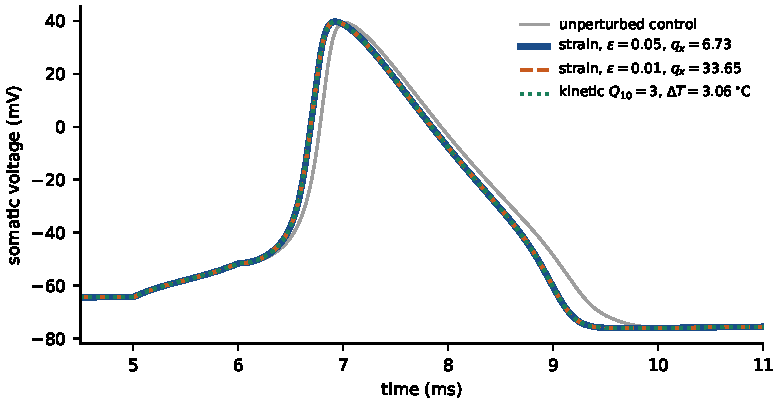
\includegraphics[width=0.72\textwidth]{fig_equivalence.pdf}
\caption{Observational equivalence within the multiplicative class. Somatic
voltage under three distinct mechanistic hypotheses that induce the same axonal
rate multipliers: reference strain ($\varepsilon=0.05$, heavy solid line), reduced
strain with higher barrier sensitivity ($\varepsilon=0.01$, dashed line), and a
purely kinetic temperature rise ($\Delta T=3.06\,^{\circ}\mathrm{C}$, dotted
line). The three traces are numerically identical and overlie one another; the
light grey trace is the unperturbed control. The effect relative to control
reaches $27.0$~mV, so the coincidence is not an artefact of a small perturbation.}
\label{fig:equiv}
\end{figure}

\subsection{Weak waveform discrimination, strong clamp discrimination}

Figure~\ref{fig:discrim} contrasts symmetric scaling with the effective-voltage
alternative. To avoid an unfair comparison we calibrate the effective-voltage
shift to reproduce the somatic spike timing of the symmetric model rather than
matching a time constant at an arbitrary voltage; this gives
$\delta=2.29$~mV. The residual waveform difference is then $7.5$~mV at maximum
against an effect size of $27.0$~mV relative to control, so whole-cell data
distinguishes the two hypotheses, but weakly, and only after the structural and
electrical parameters have been fixed independently.

Spike timing is chosen as the calibration target because it is the endpoint an
experimenter fitting whole-cell data would actually match, but it is not the
choice most favourable to the effective-voltage hypothesis, and the conclusion
does not depend on it. Minimising the maximum waveform residual directly over
$\delta$ gives $\delta=2.79$~mV and a residual of $5.9$~mV, that is $21.9\%$ of
the effect size rather than $27.8\%$. Waveform discrimination is therefore
weaker under the best available calibration of the competitor than under the
timing-matched one, so the timing-matched figure understates the degeneracy
rather than overstating it. The clamp-level separation below survives both: at
$\delta=2.79$~mV, $L_m(V)$ ranges over $[-0.152,\,0.066]$ and $L_h(V)$ over
$[-0.105,\,0.176]$, still changing sign and still nowhere near the flat
$0.336$ predicted by symmetric scaling.

The clamp-level signatures separate qualitatively. Under symmetric scaling
$L_x(V)$ is flat at $\log 1.4=0.336$ for both gates; under the timing-matched
effective-voltage model $L_m(V)$ ranges over $[-0.124,\,0.054]$ and $L_h(V)$
over $[-0.087,\,0.144]$, both changing sign within the physiological range and
differing from each other in shape. The steady-state curves are unshifted in the
first case and translated by $2.29$~mV in the second.

\begin{figure}[ht]
\centering
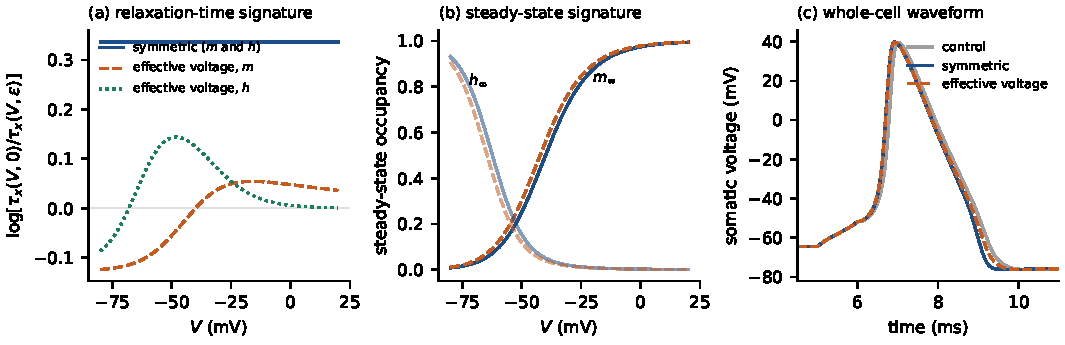
\includegraphics[width=\textwidth]{fig_discrimination.pdf}
\caption{Discriminating symmetric scaling from effective-voltage coupling, with
the effective-voltage shift calibrated to match somatic spike timing. (a)
Relaxation-time log ratio $L_x(V)$: constant and gate-independent under symmetric
scaling (solid line), voltage-dependent and gate-dependent under effective-voltage
coupling ($m$ dashed, $h$ dotted). (b) Steady-state occupancies $m_\infty$ and
$h_\infty$: unchanged under symmetric scaling (solid lines), translated under
effective-voltage coupling (dashed lines). (c) Somatic waveforms: unperturbed
control (light grey), symmetric scaling (solid) and effective-voltage coupling
(dashed). The two hypotheses nearly coincide while both depart clearly from
control, illustrating that whole-cell data discriminates weakly where clamp data
discriminates qualitatively.}
\label{fig:discrim}
\end{figure}

\subsection{Scope of the illustration}

We deliberately do not report the effect of the perturbation on onset rapidity,
compartment ordering, or threshold. By Proposition~\ref{prop:two} such
quantities are functionals of the trajectory, hence constant across the
equivalence class, hence uninformative about the mechanical hypothesis. They
characterise the consequences of localised kinetic acceleration, which is a
different and much older question \citep{brette2013}.

\section{Consequences for experimental design}
\label{sec:design}

The analysis yields a short list of constraints. They are cheap and none
requires apparatus beyond what a mechanosensitivity study already uses.

\paragraph{Clamp temperature to better than $0.31\,^{\circ}$C and report it.}
By \eqref{eq:dT}, an uncontrolled drift of $\Delta T$ accounts for a fraction
$\Delta T\log Q_{10}/(10\log\rho)$ of an observed acceleration $\rho$. If
thermal drift is to explain no more than a tenth of a reported 1.4-fold effect
at $Q_{10}=3$, temperature must be held to $0.31\,^{\circ}$C. Mechanical
stimulation by pressure or flow is not thermally neutral by default, and bath
temperature at the headstage is not the relevant quantity.

\paragraph{Measure at least two gates and report their ratio.}
By Proposition~\ref{prop:three}, the common-mode acceleration is confounded and
the gate-selective component is not. A study reporting only sodium activation
cannot distinguish its result from a uniform rate artefact. Reporting
$\rho_m/\rho_h$ against the spread of independently measured gate-specific
thermal coefficients converts a confounded observation into an identifiable one.

\paragraph{Measure $\tau_x$ across voltage, not at one voltage.}
By Proposition~\ref{prop:four}, the discriminating observable is the
\emph{constancy} of $L_x(V)$, which a single-voltage measurement cannot assess.
A systematic voltage dependence of $L_x$, or a strain-dependent translation of
$x_\infty$, rejects the symmetric barrier hypothesis and indicates coupling to
the open--closed free-energy difference rather than to the barrier alone.

\paragraph{Record peak conductance.}
By Section~\ref{sec:density}, strain and warming move $\bar g$ in opposite
directions, with a predicted divergence of $8$ to $24\%$ at the reference
perturbation depending on the conductance $Q_{10}$ and with a sign that does not
depend on it. This is the single cheapest discriminator available and it is
usually already in the data.

\paragraph{Impose at least two strain levels, and measure strain.}
By Corollary~\ref{cor:one}, one level identifies only $\eta_x$. Two or more
levels permit the assumed linearity of $\eta_x$ in $\varepsilon$ to be tested
rather than imposed. Independent estimation of $\varepsilon$ from patch geometry
is what converts $\eta_x$ into the physical coefficient $q_x$.

\paragraph{Do not treat waveform agreement as evidence.}
By Corollary~\ref{cor:two}, agreement between a strain-coupled compartmental
model and a recorded action potential is compatible with a purely thermal
perturbation of the same magnitude and carries no mechanical information.

\begin{remark}[Magnitude of the implied coupling]
The analysis says nothing about whether the reference coupling is physically
reasonable, but the identifiable quantity makes that easy to check. Writing the
barrier change as $\delta\Delta G_x^{\ddagger}=-\Delta\gamma\,\Delta
A_x^{\ddagger}$ with $\Delta\gamma=K_A\varepsilon$, the implied in-plane area
change at the transition state is
$\Delta A_x^{\ddagger}=\eta_x k_{\mathrm B}T/(K_A\varepsilon)$. For
$\eta_x=\log 1.4$, $\varepsilon=0.05$ and a bilayer area-expansion modulus
$K_A\approx0.24$~N/m \citep{evans1987}, this is $\Delta A_x^{\ddagger}\approx
0.11$~nm$^2$, rising to roughly $0.45$~nm$^2$ at a tension increment of
$3$~mN/m. These are modest values by comparison with mechanosensitive channel
gating areas. The same calculation shows that $\varepsilon=0.05$ at that modulus
corresponds to a tension increment near $12$~mN/m. Artificial bilayers and
biological membranes stretch elastically only until their area rises by some two
to three per cent, rupturing thereafter at tensions of roughly $1$ to
$12$~mN/m \citep{morris2001}, so a bilayer cannot sustain $\varepsilon=0.05$ at
all, and $\varepsilon$ in this context should be read as apparent whole-cell
areal strain, which includes unfolding of membrane reservoirs, rather than as
bilayer strain, of which such
preparations carry a substantial reservoir. Whether a given $\varepsilon$ is achievable in a given
preparation is an experimental question, and the analysis is conditional on it,
but the conditional is harmless: by Corollary~\ref{cor:one} only the product
$q_x\varepsilon$ is identifiable, so a smaller achievable strain rescales the
implied coefficient without altering any degeneracy or any discriminator. The
reference perturbation fixes a scale for the numbers quoted here; it is not a
claim about what a membrane can sustain.
\end{remark}

\section{Scope and limitations}

The equivalence result is confined to the multiplicative class $\mathcal{M}$.
Couplings that are state-dependent, that act asymmetrically on forward and
reverse rates, that alter the voltage dependence of the rate functions, or that
introduce memory, all escape Proposition~\ref{prop:two}, and the corresponding
models are correspondingly less degenerate. That is an argument for stating the
coupling class explicitly rather than an argument against symmetric scaling.

The next class up is worth naming, because it is cheap to adopt and not
degenerate in the same way. Allow the forward and reverse rates to carry
separate multipliers, $\alpha_x\mapsto\rho^{\alpha}_{x}\alpha^0_x$ and
$\beta_x\mapsto\rho^{\beta}_{x}\beta^0_x$. Proposition~\ref{prop:one} then
fails, since
\begin{equation*}
x_\infty=\frac{\rho^{\alpha}_x\alpha^0_x}
{\rho^{\alpha}_x\alpha^0_x+\rho^{\beta}_x\beta^0_x},
\end{equation*}
which reduces to the unperturbed curve only when
$\rho^{\alpha}_x=\rho^{\beta}_x$. The asymmetric part of the perturbation
therefore appears in the steady-state activation curve, where it is directly
measurable, while the symmetric part remains confounded with temperature exactly
as before. Physically this is the difference between a coupling that moves the
barrier alone and one that also moves the open--closed free-energy difference,
and it is the model to fit when the steady-state curve is observed to shift.

The thermal equivalence of Corollary~\ref{cor:two} is exact only for the kinetic
component of a temperature change. Real temperature changes also scale maximal
conductances and shift reversal potentials through the Nernst relation, and
gate-specific $Q_{10}$ values differ. Each of these breaks the degeneracy, and
each is the basis of one of the discriminators in Section~\ref{sec:design}. The
correct summary is that the kinetic and thermal hypotheses coincide exactly on
the gating equations and diverge only through effects the multiplicative
framing omits, which is precisely why omitting them is costly.

Nothing here bears on whether voltage-gated channels are mechanosensitive. That
is an experimental question with an affirmative answer in several preparations
\citep{morris2007,coste2010,murthy2017}. The claim is narrower: within the
modelling idiom most commonly used to represent the effect, a large part of the
apparent content is not identifiable, and the identifiable part is not the part
usually reported.

\section{Conclusion}

Symmetric scaling of Hodgkin--Huxley gating rates is a well-motivated minimal
coupling, and its two attractive properties, invariance of the steady-state
curve and pure rescaling of relaxation time, are exactly the properties that
make it observationally degenerate. The solution operator of an arbitrary
compartmental system depends on the perturbation only through the vector of rate
multipliers. Strain, temperature and isoform substitution can therefore be made
to coincide exactly, and a 1.4-fold acceleration is equivalent to a
$3.06\,^{\circ}$C rise at $Q_{10}=3$.

What survives is specific and testable. The gate-selective component of the
log-multiplier vector is identifiable and is not produced by uniform thermal
scaling. Symmetric scaling predicts a voltage-independent log ratio of
relaxation times together with an unshifted steady-state curve, which separates
it from effective-voltage coupling. Areal strain and warming act on channel
surface density with opposite sign. A mechanosensitivity experiment that
controls temperature tightly, measures two gates, varies voltage, records peak
conductance, and imposes more than one strain level can decide the question. One
that fits a spike waveform cannot.

\section*{Data and code availability}

The simulation code and the scripts generating both figures and all reported
numerical values are archived at Zenodo,
\url{https://doi.org/10.5281/zenodo.22828618}, and are also available from the
author.

\section*{Declaration of competing interest}

The author declares no competing interests.

\begin{thebibliography}{99}

\bibitem{bellman1970}
Bellman, R., {\AA}str{\"o}m, K.J., 1970.
On structural identifiability.
Mathematical Biosciences 7, 329--339.

\bibitem{bennetts2001}
Bennetts, B., Roberts, M.L., Bretag, A.H., Rychkov, G.Y., 2001.
Temperature dependence of human muscle ClC-1 chloride channel.
Journal of Physiology 535, 83--93.

\bibitem{brette2013}
Brette, R., 2013.
Sharpness of spike initiation in neurons explained by compartmentalization.
PLoS Computational Biology 9, e1003338.

\bibitem{chis2011}
Chi{\c s}, O.-T., Banga, J.R., Balsa-Canto, E., 2011.
Structural identifiability of systems biology models: a critical comparison of
methods.
PLoS ONE 6, e27755.

\bibitem{cobelli1980}
Cobelli, C., DiStefano, J.J., 1980.
Parameter and structural identifiability concepts and ambiguities: a critical
review and analysis.
American Journal of Physiology 239, R7--R24.

\bibitem{coste2010}
Coste, B., Mathur, J., Schmidt, M., Earley, T.J., Ranade, S., Petrus, M.J.,
Dubin, A.E., Patapoutian, A., 2010.
Piezo1 and Piezo2 are essential components of distinct mechanically activated
cation channels.
Science 330, 55--60.

\bibitem{evans1987}
Evans, E., Needham, D., 1987.
Physical properties of surfactant bilayer membranes: thermal transitions,
elasticity, rigidity, cohesion, and colloidal interactions.
Journal of Physical Chemistry 91, 4219--4228.

\bibitem{eyring1935}
Eyring, H., 1935.
The activated complex in chemical reactions.
Journal of Chemical Physics 3, 107--115.

\bibitem{frankenhaeuser1963}
Frankenhaeuser, B., Moore, L.E., 1963.
The effect of temperature on the sodium and potassium permeability changes in
myelinated nerve fibres of \emph{Xenopus laevis}.
Journal of Physiology 169, 431--437.

\bibitem{hodgkin1952}
Hodgkin, A.L., Huxley, A.F., 1952.
A quantitative description of membrane current and its application to conduction
and excitation in nerve.
Journal of Physiology 117, 500--544.

\bibitem{morris2001}
Morris, C.E., Homann, U., 2001.
Cell surface area regulation and membrane tension.
Journal of Membrane Biology 179, 79--102.

\bibitem{morris2007}
Morris, C.E., Juranka, P.F., 2007.
Nav channel mechanosensitivity: activation and inactivation accelerate
reversibly with stretch.
Biophysical Journal 93, 822--833.

\bibitem{murthy2017}
Murthy, S.E., Dubin, A.E., Patapoutian, A., 2017.
Piezos thrive under pressure: mechanically activated ion channels in health and
disease.
Nature Reviews Molecular Cell Biology 18, 771--783.

\bibitem{schwarz1986}
Schwarz, J.R., 1986.
The effect of temperature on Na currents in rat myelinated nerve fibres.
Pfl\"ugers Archiv 406, 397--404.

\bibitem{sukharev2012}
Sukharev, S., Sachs, F., 2012.
Molecular force transduction by ion channels: diversity and unifying principles.
Journal of Cell Science 125, 3075--3083.

\bibitem{walch2016}
Walch, O.J., Eisenberg, M.C., 2016.
Parameter identifiability and identifiable combinations in generalized
Hodgkin--Huxley models.
Neurocomputing 199, 137--143.

\end{thebibliography}

\end{document}
